\documentclass[letterpaper,11pt]{article}
\usepackage{graphicx}
\usepackage{listings}
\usepackage[super]{nth}
\usepackage[hyphens]{url}
\usepackage{hyperref}
\usepackage{amsmath}
\usepackage[makeroom]{cancel}
\usepackage[table]{xcolor}
\usepackage{comment}
\usepackage[space]{grffile}



\lstset{
numbers=left,
backgroundcolor=\color{white},
frame=single,
tabsize=2,
captionpos=b,
breaklines=true,
breakautoindent=true,
escapeinside={\%*}{*)}
}

\begin{document}

\begin{titlepage}

\begin{center}

\Huge{Assignment 4}

\Large{CS 532:  Introduction to Web Science}

\Large{Spring 2018}

\Large{Chandrasekhar Reddy Muthyala}

\Large Finished on \today

\end{center}

\end{titlepage}

\newpage


% =================================
% First question
% =================================
\section*{1}


\subsection*{Question}



\begin{verbatim}
The "friendship paradox" (http://en.wikipedia.org/wiki/Friendship_paradox)
says that your friends have more friends than you do.  

1.  Determine if the friendship paradox holds for my Facebook
account.* Compute the mean, standard deviation, and median of the
number of friends that my friends have.  Create a graph of the
number of friends (y-axis) and the friends themselves, sorted by
number of friends (y-axis).  (The friends don't need to be labeled
on the x-axis: just f1, f2, f3, ... fn.)  Do include me in the graph
and label me accordingly.

* = This used to be more interesting when you could more easily download
your friend's friends data from Facebook.  Facebook now requires each
friend to approve this operation, effectively making it impossible.

I will upload a csv file of my 2014 friends list on the #assignment-4 slack channel
\end{verbatim}


\clearpage
\subsection*{Answer}

To solve this problem I have gone through the above link and understood what friendship paradox is, and started writing a programming in python \textbf{friendsParadox.py}  for displaying friendship paradox graph for Prof. anwala’s Facebook account. Prof. anwala gave his facebook friends of friends count in \textbf{acnwala-friendscount.csv}.\\
List of python dependency libraries
\begin{itemize}
    \item import matplotlib.pyplot as plt
    \item import pandas as pd
    \item import numpy as np
    \item import math
\end{itemize}
Initially in the program I am reading a csv using pandas and it will convert into data frame. From that data frame I took friends count column and converted in to list \textbf{y\_axis} that acts as y-axis. Using that list length I have created a \textbf{x\_axis} list to indicate number of friends. First Using numpy library I calculated mean, median and standard deviation (SD) and appending into y\_axis list to plot the mark on the graph. I took \textbf{myFriends} variable which will store prof. Anwal’s friends count and appending into y\_axis list just like mean, median and SD to plot where Prof. anwala stands in the graph whether above or below mean and median values. 
\subsection*{Run on the command line}
\begin{lstlisting}[frame=single]
python friendsParadox.py
\end{lstlisting}
\lstinputlisting[frame=single,caption={Python script for ploting friends paradox for Facebook account },label=lst:q1tweepy,captionpos=b,numbers=left,showspaces=false,breakindent=0.5pt,showstringspaces=false,basicstyle=\footnotesize]{friendsParadox.py}

 In the plot shown in below  Figure , you can see that Prof.Anwala has many friends with higher friend counts than him, with his count being 98 (not including himself). Therefore, the friendship paradox does hold for Prof.Anwala's Facebook account. I also used this Python script to compute the Mean, Standard Deviation and Median of Prof.Anwala's Facebook friend counts shown in Table.

\begin{table}[htb]
\centering
\begin{tabular}{ | l | l | l |}
\hline
\textbf{Mean} & \textbf{Standard Deviation} & \textbf{Median} \\
\hline
542.67 & 536.67 & 396.0\\
\hline
\end{tabular}
\caption{Mean, Standard Deviation and Median generated from Python  Script for Facebook friend counts}
\label{table:q1summary}
\end{table}
\clearpage
\begin{figure}[h]
\centering
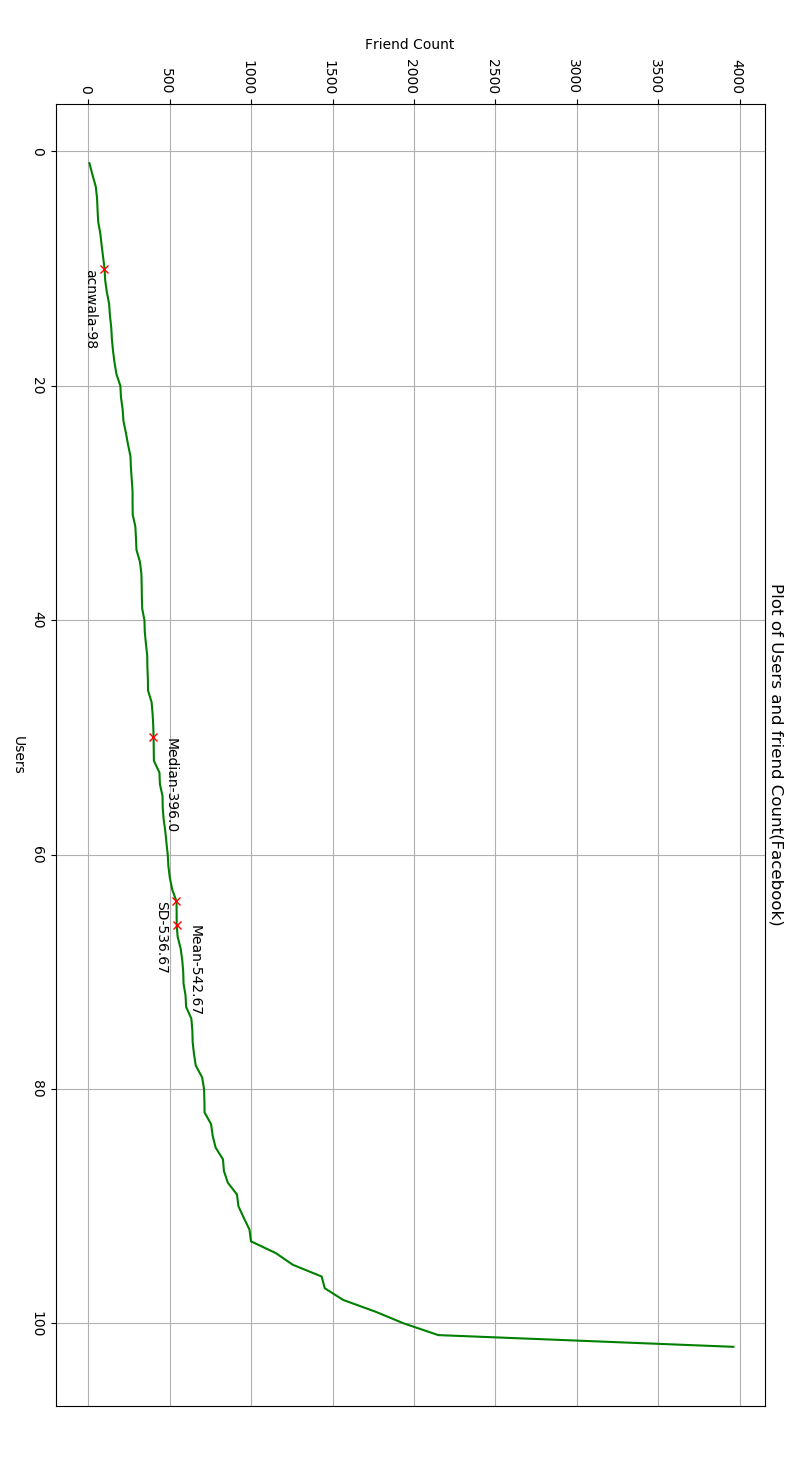
\includegraphics[scale=0.6]{facebookPlot.png} 
\caption{Plot of Prof.Anwala's Facebook friends vs. friend counts}
\label{fig:q1facebookplot}
\end{figure}}

\clearpage

% =================================
% Second question
% =================================

\section*{2}

\subsection*{Question}

\begin{verbatim}
2.  Determine if the friendship paradox holds for your Twitter account.
Since Twitter is a directed graph, use "followers" as value you measure
(i.e., "do your followers have more followers than you?").

Generate the same graph as in question #1, and calcuate the same 
mean, standard deviation, and median values.

For the Twitter 1.1 API to help gather this data, see:

https://developer.twitter.com/en/docs/accounts-and-users/follow-search-get-users

If you do not have followers on Twitter (or don't have more than 50),
then use my twitter account "acnwala".

\end{verbatim}

\clearpage
\subsection*{Answer}

To solve this problem I have gone through the twitter API Tweepy and found one solution for getting followings and followers based on the screen name given to that API. There is a cursor function in tweepy library  to get details of friends of friends in twitter. 
For this problem I am passing screen name and variable which I wanted to  extracting from my friends account let say  in this problem I want following count of  my friends (that is whom I am following in twitter).  I am saving screen name of my friends and their corresponding following count in \textbf{friendsCount.csv} file, like wise for followers of my followers I am passing followers and screen name to the cursor function which will give me count of my flowers of followers count ad storing in \textbf{followersCount.csv} file. I have collected data for problem\#2 in \textbf{friendsCount.csv} and problem\#4 in \textbf{followersCount.csv} to plot friendship paradox.\\
List of python dependency libraries to extract above data

\begin{itemize}
    \item import tweepy
    \item import csv
\end{itemize}
\subsection*{Run on the command line}
\begin{lstlisting}[frame=single]
python friendsofFriendsFromTwitter.py
\end{lstlisting}
\lstinputlisting[frame=single,caption={Python script for extracting friends and followers of friends from twitter },label=lst:q1tweepy,captionpos=b,numbers=left,showspaces=false,breakindent=0.5pt,showstringspaces=false,basicstyle=\footnotesize]{friendsofFriendsFromTwitter.py}
To draw the friendship paradox of twitter friends I wrote a program just like problem\#1 named as \textbf{twitterFriendsParadox.py}
\subsection*{Run on the command line}
\begin{lstlisting}[frame=single]
python twitterFriendsParadox.py
\end{lstlisting}
\lstinputlisting[frame=single,caption={Python script for generating a plot  Twitter Friends Of friends Of  Hemanth Malla},label=lst:q1tweepy,captionpos=b,numbers=left,showspaces=false,breakindent=0.5pt,showstringspaces=false,basicstyle=\footnotesize]{twitterFriendsParadox.py}
\clearpage
\begin{table}[htb]
\centering
\begin{tabular}{ | l | l | l |}
\hline
\textbf{Mean} & \textbf{Standard Deviation} & \textbf{Median} \\
\hline
820.14 & 2359.61 & 324 \\
\hline
\end{tabular}
\caption{Mean, Standard Deviation and Median generated from python Script for twitter follower count}
\label{table:q2summary}
\end{table}
In the plot shown in below  Figure , you can see that Hemanth malla has many friends with higher friend counts than him, with his count being 746 (not including himself). Therefore, the friendship paradox does hold for Hemanth malla's Twitter account.
\begin{figure}[h]
\centering
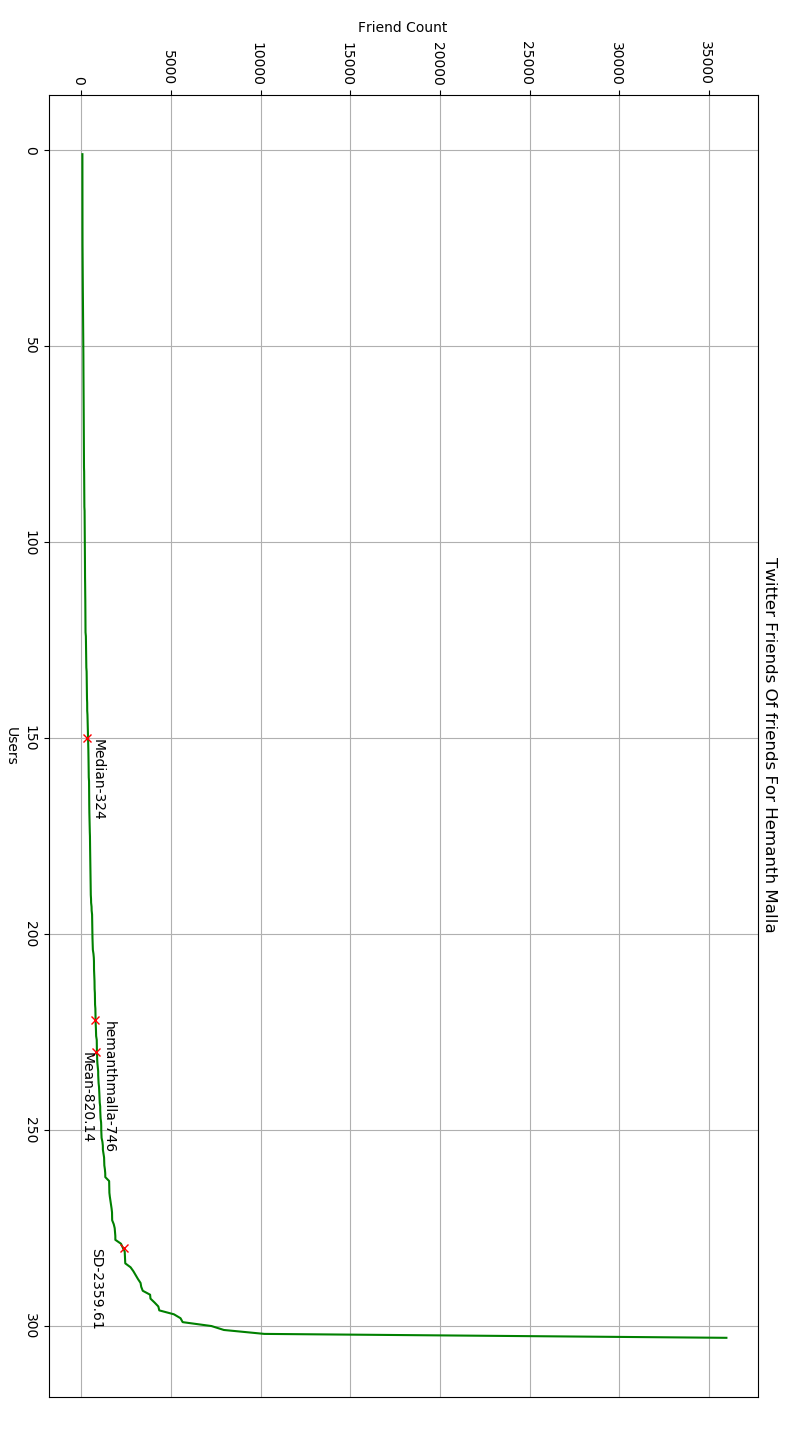
\includegraphics[width=\textwidth]{twitterFriendsParadox.png}
\caption{Plot of Hemanth malla's Twitter friends vs. friends counts}
\label{fig:q2followers}
\end{figure}


\lstinputlisting[frame=single,caption={Python script for receiving twitter followers and friends from  Hemanth malla's twitter},label=lst:twitterpy,captionpos=b,numbers=left,showspaces=false,showstringspaces=false,basicstyle=\footnotesize]{\srcPath/twitterFriendship.py}

\clearpage

% =================================
% Third question
% =================================

\section*{3}

\subsection*{Question}

\begin{verbatim}
Extra credit, 1 point:

3.  Repeat question #1, but with your (or a specified) LinkedIn profile.
\end{verbatim}

\clearpage
\subsection*{Answer}

To solve this problem I have gone through LinkedIn api for developers documentation, after gone through the documentation I understood that developers account is to get the basic information of my own profile and it is not providing any information of my connections profile. There is REST Console to check the api, when I tested it on the console by hitting the below URL I got below json as a result.
\begin{lstlisting}[frame=single]
https://api.linkedin.com/v1/people/~?format=json
\end{lstlisting}
\begin{lstlisting}[frame=single]
{
  "firstName": "Chandra Sekhar Reddy",
  "headline": "Actively seeking Summer Internship.",
  "id": "ieRtV_6P-3",
  "lastName": "muthyala",
  "siteStandardProfileRequest": {"url": "https://www.linkedin.com/profile/view?id=AAoAABAxil4Bvywspn9jEWbxrqYnUoABFEL_rYE&authType=name&authToken=yJSt&trk=api*a3227641*s3301901*"}
}
\end{lstlisting}
\clearpage

% =================================
% Fourth question
% =================================

\section*{4}

\subsection*{Question}

\begin{verbatim}
4.  Repeat question #2, but change "followers" to "following"?  In
other words, are the people I am following following more people?

For the Twitter 1.1 API to help gather this data, see:

https://developer.twitter.com/en/docs/accounts-and-users/follow-search-get-users/
\end{verbatim}

\clearpage
\subsection*{Answer}

To solve this problem, we got data for this problem from \textbf{friendsofFriendsFromTwitter.py”} and stored in \textbf{followersCount.csv} file.

To draw the friendship paradox of twitter followers of my screen name followers I wrote a program just like problem\#1 named as \textbf{twitterFriendsParadox.py}
\subsection*{Run on the command line}
\begin{lstlisting}[frame=single]
pythontwitterFollowersParadox.py
\end{lstlisting}
\lstinputlisting[frame=single,caption={Python Script for generating plot Twitter Followers Of Followers Of  Hemanth Malla},label=lst:q3rscript,captionpos=b,numbers=left,showspaces=false,showstringspaces=false,basicstyle=\footnotesize]{twitterFollowersParadox.py}
\begin{table}[htb]
\centering
\begin{tabular}{ | l | l | l |}
\hline
\textbf{Mean} & \textbf{Standard Deviation} & \textbf{Median} \\
\hline
5643.14 & 42238.58 & 155 \\
\hline
\end{tabular}
\caption{Mean, Standard Deviation and Median generated from python Script for twitter following count}
\label{table:summaryExtra}
\end{table}
In the plot shown in below  Figure , you can see that Hemanth malla has many Followers with higher Follwers counts than him, with his count being 193 (not including himself). Therefore, the friendship paradox does hold for Hemanth malla's Twitter account.
\begin{figure}[h]
\centering
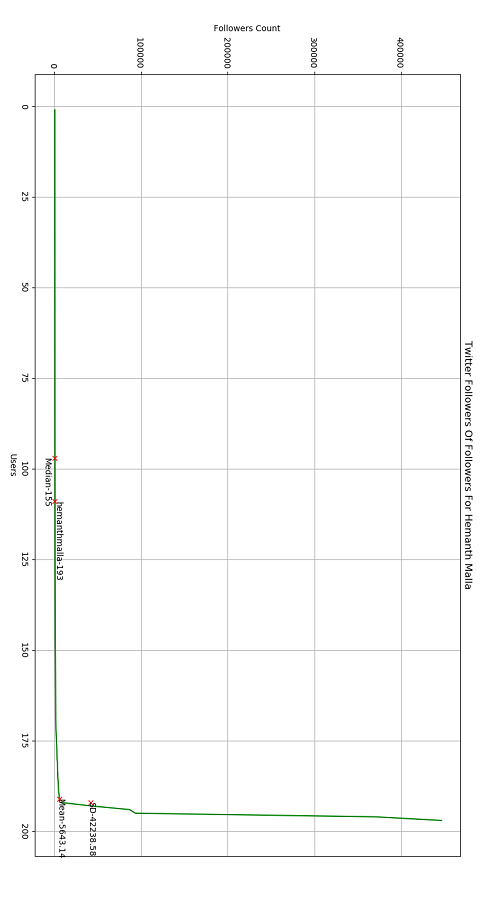
\includegraphics[scale=1.0]{twitterFollowersParadox.png}
\caption{ plot of Hemanth malla's Facebook Twitter following vs. following counts}
\label{fig:scatterplot}
\end{figure}
\clearpage
% =================================
% Bibliography
% =================================

\begin{thebibliography}{9}

\bibitem{LinkedInapi} \url{https://developer.linkedin.com/docs/rest-api}.
\bibitem{twitterapi}
``Twitter Developer Documentation''. Twitter. Twitter, n.d. Web. 1 March 2017. \url{https://dev.twitter.com/rest/reference/get/followers/list}.
\end{thebibliography}

\end{document}